\setcounter{secnumdepth}{3} 

\chapter{On the Risk of Systematic Drift Under Incoherent Hierarchical Forest Management Planning}

This chapter presents an article entitled \emph{On the Risk of Systematic Drift Under Incoherent Hierarchical Forest Management Planning}, published in the \emph{Canadian Journal of Forest Research}, 43(5):480--492, 2013. The authours are Gregory Paradis, Luc LeBel, Sophie D'Amours, and Mathieu Bouchard.

\pagebreak

\selectlanguage{francais}

\begin{abstract}
    En th\'{e}orie, les syst\`{e}mes de planification hi\'{e}rarchiques
  int\`{e}grent des m\'{e}canismes de liaison efficaces, assurant ainsi
  une d\'{e}saggr\'{e}gation coh\'{e}rente de l'attribution de volumes
  aux usines lors de la planification d\'{e}taill\'{e}e des
  op\'{e}rations de r\'{e}colte. En pratique, les m\'{e}canismes de
  liaison entre la planification \`{a} long- et \`{a} court-terme
  peuvent \^{e}tre inefficaces, menant donc \`{a} des plans
  incoh\'{e}rents en termes du volume r\'{e}colt\'{e}, de la
  repr\'{e}sentation des essences, et du potentiel de cr\'{e}ation de
  valeur des billes livr\'{e}es aux usines. Cette incoh\'{e}rence
  entre la planification et l'ex\'{e}cution de la r\'{e}colte peut
  induire une d\'{e}rive syst\'{e}matique de l'\'{e}tat du syst\`{e}me
  forestier (c.-\`{a}-d. divergence entre les trajectoires
  projet\'{e}es et r\'{e}alis\'{e}es), compromettant donc la
  cr\'{e}dibilit\'{e} et la performance du processus de planification
  de l'am\'{e}nagement forestier.

  Nous d\'{e}crivons le processus de planification foresti\`{e}re en
  termes de la th\'{e}orie du jeu, et nous simulons l'interaction
  entre la planification de l'approvisionnement et la planification de
  la r\'{e}colte \`{a} l'aide d'un mod\`{e}le it\'{e}ratif \`{a} deux
  phases. Nous pr\'{e}sentons une \'{e}tude de cas, et nous montrons
  l'existence d'un effet de d\'{e}rive syst\'{e}matique, que nous
  attribuons \`{a} l'innefficacit\'{e} des m\'{e}canismes reliant la
  planification à long- et à court-terme. Nous montrons qu'il est
  possible d'am\'{e}liorer la coh\'{e}rence des plans en manipulant
  les m\'{e}canismes de liaison, et proposons des avenues de recherche
  futures pouvant potentiellement am\'{e}liorer la performance du
  processus de planification hi\'{e}rarchique \`{a} l'aide de
  nouvelles formulations de mod\`{e}les bas\'{e}s sur la th\'{e}orie
  du jeu.
\end{abstract}

%\pagebreak

\selectlanguage{english}

\begin{abstract}
  In theory, linkages between hierarchical forest management planning
  levels ensure coherent dis-aggregation of long-term wood supply
  allocation as input for short-term demand-driven harvest
  planning. In practice, these linkages may be ineffective, and
  solutions produced may be incoherent in terms of volume and value
  creation potential of harvested timber. Systematic incoherence
  between planned and implemented forest management activities may
  induce drift of forest system state (ie.  divergence of planned and
  actual system state trajectories), thus compromising credibility and
  performance of the forest management planning process.

  We describe hierarchical forest management from a game-theoretic
  perspective, and present an iterative two-phase model simulating
  interaction between long- and short-term planning processes. Using
  an illustrative case study, we confirm the existence of a systematic
  drift effect, which we attribute to ineffective linkages between
  long- and short-term planning. In several simulated scenarios,
  the planning process fails to ensure long-term wood supply
  sustainability, fails to reliably meet industrial fiber demand over
  time, and exacerbates incoherence between wood supply and fiber
  demand over several planning iterations. We show that manipulating
  linkages between long- and short-term planning processes can reduce
  incoherence, and describe future work on game-theoretic planning
  process model formulations that may improve hierarchical planning
  process performance.
\end{abstract}

\pagebreak

\section{Introduction}

Hierarchical forest management (HFM) on public land may currently be
failing on two levels. At the top level, HFM may not be providing
credible assurance of long-term sustainability of timber supply and
forest ecosystem integrity. At a lower level, HFM may be failing to
fully realize value-creation potential from timber-harvesting
activities through over-constraining of the harvest planning
problem. These failures can be traced back to unrealistic assumptions
regarding long-term timber consumption behaviour. These problematic
assumptions are implicitly embedded into the optimization models used
to determine annual allowable cut (AAC) levels, which may explain
why this problem has received little attention in the literature.

Operations research (OR) has been used extensively in forest resource
planning in the past several decades \citep{weintraub2006operations}.
Many forestry applications of OR are developed in a hierarchical
planning framework \citep{weintraub1991hierarchical,
  weintraub2007handbook}. Justification for hierarchical decomposition
of planning problems is based on problem size, correspondence of
solution decision levels to organizational structure, and simplicity
of planning approach in a realistic forest planning context
\citep{weintraub1991hierarchical}.  However, decomposing a planning
problem into a hierarchy of planning levels introduces risk of
distorting global solution space.  Thus, hierarchical planning systems
may produce globally infeasible or globally sub-optimal solutions.

Forestry applications of OR in the literature have
tended to focus on either forest management issues (eg. sustainability
of timber and non-timber forest values, land use allocation,
silvicultural strategies, etc.)
\citep{bettinger2004key,gunn2007models} or on forest products industry
supply-chain planning \citep{damours2008using,carlsson2006supply}.
Nevertheless, obvious interdependencies exist between long-term forest
management planning and short-term forest industry supply chain
planning.  In particular, coherence of long- and short-term
planning is highly dependent on assumptions regarding the relationship
between supply and demand, and assumptions regarding the spatial
distribution of harvesting activities. Relatively little research has been
published on integration of forest management planning and forest
products industry supply chain planning, although several interesting
research topics in this area are described in \citet{nelson2003forest}
and \citet{weintraub2006review}.  Recent publications
\citep{troncoso2011mixed,gunn2009some} indicate some recent and
ongoing work integrating strategic wood supply analysis and supply
chain planning. 

We believe improved integration of long-term wood supply planning and
short-term fiber demand planning is key to improving the
performance and credibility of the hierarchical forest management
planning process. Throughout this paper, we use the terms
\emph{performance} and \emph{credibility} in reference to the
hierarchical forest management planning process. We use the term
\emph{performance} to describe the realization of value-creation
potential, and the term \emph{credibility} to describe extent to which
assurance of long-term sustainability is supported by currently
available information (ie. believable). Usage of the term
\emph{credibility} in this context is coherent with usage in
\citet{daugherty1991credibility} and \citet{davis2001forest-ch13}.

A key component of the hierarchical planning paradigm is the existence of
effective linkages between planning levels \citep{bitran1977design}.
These linkages should ensure coherence between hierarchical planning
levels, and limit risk of introducing distortions in solution
space. In practice, execution of a hierarchical forest planning
process tends to be distributed across teams of planners with stable,
but divergent, planning objectives. Planning levels are typically
linked by several constraints, including allowable cut levels and
operational harvesting regulations.  Furthermore, strategic plans are
reviewed every few years. Nonetheless, existing linkages combined with a
regular re-planning cycle may not fully correct biases induced by systematic
differences between planned and implemented activities. More
specifically, improperly designed linkages between planning levels may
be distorting solutions, producing long-term projections that are
systematically biased relative to as-implemented course of
action. The long-term impact, on forest system state, of systematic bias
between planned and implemented forest harvesting activities is
largely unknown, and has received relatively little attention in the
literature
\citep{bettinger2004key,weintraub2006operations,pittman2007hierarchical}.

\citet{daugherty1991credibility} explored \emph{dynamic inconsistency}
in forest planning based on linear programming (LP) using an iterative
linear programming simulation of sequential re-planning, assuming
exact implementation of first-period optimal solution at each
iteration, discounted profit-maximization objective function, and
even-flow harvest volume constraints.  He argued that maximizing
discounted profit in conjunction with even-flow constraints creates
dynamically inconsistent long-term model formulations, which are not a
credible basis for near-term policy decisions, and notes that dynamic
inconsistency in long-term models may be avoidable using alternative
objective function formulations or different harvest flow control
approaches. \citet{mcquillan1986declining} makes similar observations,
also based on long-term model formulations featuring discounted
profit-maximization objective functions and even-flow harvest volume
constraints.

Strategic forest planning on public forest tends to focus on
establishing timber resource allocation such that long-term
sustainability constraints are respected. An important component of
strategic forest planning in several jurisdictions is annual allowable
cut level calculation, often based on complex simulations of forest
growth and projected management activity levels. The current purpose
of AAC determination within the forest management planning process is
twofold: to ensure long-term sustainability of the timber supply, and to
demonstrate long-term integrity of the forest ecosystem.

It is common practice to maximize AAC through optimal scheduling of
forest management activities, using an aggregate representation of the
forest landscape. In this context, validity of AAC projections depends
on validity of model assumptions regarding current and future harvest
levels, spatial distribution of harvest areas on forest landscape, and
silviculture activity levels. These long-term projections are only
valid under specific conditions, \emph{viz. (a) }model is dynamically
consistent, \emph{(b)} first period of optimal AAC solution is implemented exactly and
\emph{(c)} deterministic assumptions regarding forest inventory,
forest growth, and silviculture treatment effects hold true. Thus,
the credibility of long-term AAC solutions as a basis for short-term policy
decisions depends on the extent to which these validity conditions are
respected.  If implemented forest management activities differ
significantly from activities simulated by AAC models, then the AAC
modelling process is unlikely to provide credible information
regarding the sustainability of wood supply or the integrity of forest
ecosystems. Regardless of credibility level, AAC solutions always
constrain short-term harvest planning solution space, thereby
potentially limiting short-term value-creation opportunities induced
by timber harvesting activities. Constraining short-term
value-creation opportunities on the basis of low-credibility long-term
projections is of questionable merit, and limits the rationality of
the forest management policy decision-making process.

At the short-term harvest planning level, AAC is typically interpreted
as an upper bound on the allowable harvest level; short-term harvest plans
may include any subset of AAC. This interpretation of AAC does not
respect one of the solution validity conditions described earlier
(ie. optimal AAC solution is implemented exactly). In practice,
implemented harvest level may be significantly lower than AAC if
\emph{(a)} aggregate timber demand is lower than AAC, \emph{(b)}
composition of harvested stands in AAC model is incoherent with timber
demand (eg. no local market for certain species-product combinations),
or \emph{(c)} portions of projected AAC harvest volume are
economically or operationally unattractive. Hence, long-term planning
models tend to systematically over-estimate current and future harvest
and silviculture activity levels, and short-term harvesting plans tend
to distort long-term planning assumptions in favour of demand
satisfaction and cost minimization (or profit maximization).

If left unresolved, this biased incoherence between planned and
implemented harvest and silviculture activity levels may induce
systematic drift of the forest system state (ie. long term trajectory
of system state systematically differs from projected system state)
after several iterations of implementing incoherent strategic and
operational plans, thus reducing the credibility of long-term planning
effort and potentially over-constraining short-term value-creation
opportunity. This \emph{systematic drift effect} (SDE), induced by
incoherence between hierarchical forest planning levels, is not
discussed in the literature. The objectives of this paper are: to
examine the impact of \emph{status quo} hierarchical decomposition of
forest management planning on the performance and credibility of the
overall planning process using the SDE concept as a basis for
evaluation, to identify weaknesses in the linkages between planning
levels, to simulate SDE using an illustrative case study, and to
propose potential improvements to the planning process.

% The structure of this paper is as follows. Problem definition is
% presented in \S \ref{sec:problem}. Model formulation is presented in
% \S \ref{sec:model}, and test dataset is described in \S
% \ref{sec:dataset}. Experimental design is described in \S
% \ref{sec:experiment}, and experimental results are presented in \S
% \ref{sec:results}. Finally, discussion and conclusion are presented in
% \S \ref{sec:discussion} and \S \ref{sec:conclusion}.

\section{Problem Definition}
\label{sec:problem}

% Hierarchical forest management is a complex and difficult problem.  
In many jurisdictions, responsibility for long-term and short-term
planning on public forest is distributed across government and
industrial agents with divergent planning objectives. Long-term wood
supply planning is typically implemented first by government planners,
followed by short-term demand-driven harvest planning by industry
planners. We model this distributed hierarchical
planning process, with the purpose of approximating the net effect of a
two-phase planning hierarchy in a rolling-horizon re-planning
context. More specifically, we examine the credibility of long-term
planning projections under varying levels of incoherence between
timber supply and demand.

We present several assumptions about the hierarchical forest
management planning process, which reflect our understanding of the
current situation in several jurisdictions where public forests are
managed by government stewards for production of timber resources:
\begin{itemize}
\item long-term planning is the responsibility of government planners (stewards
of public land);
\item short-term harvest planning is the responsibility of forest industry
planners;
\item the objective of long-term planning is to ensure long-term sustainability
of timber supply and to demonstrate long-term integrity of forest
ecosystem;
\item output from the long-term planning process includes species-wise AAC (ie.
upper bounds on species-wise harvest levels), and treatment-wise minimum
area thresholds on annual silviculture treatments;
\item the long-term AAC model is formulated as an aspatial (ie. stratum-based)
species-wise even-flow harvest maximization problem;
\item the objective of short-term harvest planning is to satisfy timber demand
at maximum profit. 
\end{itemize}

We present an illustrative case study showing that
incoherence between long- and short-term forest management planning
can negatively impact credibility and performance of the
planning process. In a worst-case scenario, incoherent planning may
induce sudden (unforeseen) wood supply failure. Alternatively,
incoherent hierarchical planning may over-constrain the short-term
planning process, impeding realization of full value-creation
potential.  In certain jurisdictions, realization of full sustainable
value-creation potential may be key to navigating periods of economic
crisis in the forest industry. We also show that extending the
\emph{status quo} long-term planning model to explicitly anticipate
certain aspects of the short-term planning process (ie. fiber demand)
can improve credibility and performance of the 
hierarchical planning process.

The remaining subsections of the problem definition describe
\emph{status quo} long- and short-term planning processes, and present
the distributed hierarchical forest management problem from a
game-theoretic perspective.

\subsection{Long-term Planning Process}

\label{sec:strategic-effectiveness}

Strategic planning on public forest land traditionally focuses on
establishing forest resource allocation (with emphasis on timber
resource) such that long-term sustainability objectives are respected
\citep{gunn2007models,davis2001forest-ch11}.  An important component of
strategic forest planning is annual allowable cut level
calculation, based on complex simulations of forest growth and
projected management activities, over a long planning horizon (eg. 150
years). AAC is often defined as maximum even-flow (species-wise)
timber harvest level on a given land base.  Despite its widespread use,
this model formulation may induce incoherence between stated
management goals and planning process outcome, especially when
long-term planning is integrated with supply chain planning
\citep{gunn2009some}.  The purpose of AAC calculation in the planning
process is to ensure long-term sustainability of the timber resource,
however sustainability is not necessarily ensured by a non-declining yield
AAC model formulation \citep{gunn2009some}.  Actual harvest levels may
fluctuate significantly from one planning period to another, and tend
to be significantly lower than harvest levels simulated by AAC models,
therefore a non-declining yield AAC model is not likely to provide a
credible projection of either future harvest levels or future forest
system state. Furthermore, maximizing even-flow AAC level through
optimal allocation of harvesting activities over time does not
guarantee efficient tradeoff between availability of timber and other
values (ie. economic, social, ecological, etc).

In fact, AAC maximization tends to rely on an \emph{allowable cut effect}
(ACE) to justify potentially unsustainable AAC simulations
\citep{luckert1995allowable}. ACE can be defined as the allocation of
anticipated future timber yields to current harvest levels, and is
used to justify increases in AAC. Depending on initial age-class
structure of the forest under management, ACE may also induce AAC
models to prescribe large short-term investments to establish
high-yield plantations to obtain marginal long-term increase in
(simulated) available timber at a critical period. These silvicultural
investments may be difficult to justify economically, especially if
anticipated harvest level is significantly lower than AAC.

The validity of AAC projections depends on the validity of underlying
assumptions regarding harvest levels, distribution of harvest areas the on
forest landscape, and other silviculture activity levels
(eg. establishment of high-yield plantations, stand improvement
treatments, etc.). AAC scenarios accurately predict future forest
conditions only  if projected harvest levels represent an \emph{unbiased}
approximation of future management activity levels.

In practice, AAC constitutes a starting point for a political
negotiation process between stewards of public forest and industrial
consumers of timber from public forest. Aggregation of forest
inventory data into stratum-based representations (ie. failure to
account for spatially-explicit operational constraints associated with
harvest block layout and landscape planning), lack of integration with
industrial fiber demand planning, and use of an ACE as a basis for
determining short-term silviculture and harvesting policy tends to
produce AAC estimations that are systematically higher than observed
harvest levels \citep{ccfm2005wood}. Although spatial disaggregation
and additional planning constraints at lower planning levels can
restore feasibility, harvest levels tend to drop on the order of 20\%,
relative to AAC, following spatially explicit feasible allocation of
harvest operations on the landscape \citep{walters2001empirical}. It
is not clear how this feasibility-restoration process impacts global
optimality, nor is it clear that strategic planning objectives
(ie. sustainability) are respected after operational feasibility
adjustment. Species-wise AAC levels are linked (due to harvesting of
multiple species in mixed stands), and sustainability is not
guaranteed for all possible combinations of species-wise harvest
levels, even if AAC upper-bound harvest constraints are
respected. Upper-bound harvest level constraints (as defined by AAC)
may be neither sufficient nor necessary to ensure long-term
sustainability of timber harvest or ecological integrity.

Table \ref{tab:harvestcontrol} compares recent AAC and harvest volume,
by province, in Canada. Actual harvest levels are in many cases
significantly lower than projected harvest levels, where actual timber
demand differs significantly from projected timber demand.  Also note
that the proportion of hardwood AAC harvested is systematically lower than the
proportion of softwood AAC harvested, indicating that the AAC
determination process simulates harvest intensity and distribution
that is unrepresentative of actual harvesting activities.  Lower
historical hardwood harvesting levels are likely linked to bounded
economic viability of hardwood fiber utilization
opportunities. Factors contributing to limit hardwood harvesting
value-creation opportunities include significant differences between
supply and demand (species distribution, quality distribution), high
unit cost of partial cut harvesting operations, and increased
dispersion and fragmentation of harvest blocks due to spatial layout
of partial cutting blocks (proportionally higher setup costs, road
construction cost, transportation cost). In some areas, only the most
valuable hardwood logs (eg. veneer grade) are economically viable
given current local market conditions, while other hardwood
co-products are harvested at a net loss.
%\citep{optivert2007calcul}.



\begin{table}[H]
\caption{Comparison of recent AAC and harvested volume, by species
(softwood, hardwood) and Canadian province \citep{ccfm2005wood}}
\label{tab:harvestcontrol}
\renewcommand{\tabcolsep}{4pt}
\begin{tabular}{lrrrrrrrrrrr}
\toprule
 & \emph{Units} & \emph{NL} & \emph{PE} & \emph{NS} & \emph{NB} & \emph{QC} & \emph{ON} & \emph{MB} & \emph{SK} & \emph{AB} & \emph{BC}\tabularnewline
\midrule
\textbf{\small Softwood} &  &  &  &  &  &  &  &  &  &  & \tabularnewline
{\small Harvest} & {\small thousand $m^{3}$} & {\small 1958} & {\small 431} & {\small 562} & {\small 3712} & {\small 24 702} & {\small 16 568} & {\small 1563} & {\small 2259} & {\small 12 090} & {\small 64 941}\tabularnewline
{\small AAC} & {\small thousand $m^{3}$} & {\small 2573} & {\small 300} & {\small 865} & {\small 3686} & {\small 31 602} & {\small 22 887} & {\small 5639} & {\small 3864} & {\small 13670} & {\small 66 653}\tabularnewline
{\small Deviation} & {\small thousand $m^{3}$} & {\small -615} & {\small +131} & {\small -303} & {\small +26} & {\small -6900} & {\small -6319} & {\small -4076} & {\small -1605} & {\small -1580} & {\small -1713}\tabularnewline
{\small Ratio} & {\small \%} & {\small 76} & {\small 144} & {\small 65} & {\small 101} & {\small 78} & {\small 72} & {\small 28} & {\small 58} & {\small 88} & {\small 97}\tabularnewline
\textbf{\small Hardwood} &  &  &  &  &  &  &  &  &  &  & \tabularnewline
{\small Harvest} & {\small thousand $m^{3}$} & {\small 62} & {\small 151} & {\small 99} & {\small 1457} & {\small 4132} & {\small 4406} & {\small 638} & {\small 1313} & {\small 6100} & {\small 1199}\tabularnewline
{\small AAC} & {\small thousand $m^{3}$} & {\small N/A} & {\small 169} & {\small 455} & {\small 1633} & {\small 12 084} & {\small 13 058} & {\small 3261} & {\small 3244} & {\small 10 210} & {\small 2843}\tabularnewline
{\small Deviation} & {\small thousand $m^{3}$} & {\small N/A} & {\small -9} & {\small -356} & {\small -176} & {\small -7952} & {\small -8652} & {\small -2623} & {\small -1931} & {\small -4110} & {\small -1645}\tabularnewline
{\small Ratio} & {\small \%} & {\small N/A} & {\small 94} & {\small 22} & {\small 89} & {\small 34} & {\small 34} & {\small 20} & {\small 40} & {\small 60} & {\small 42}\tabularnewline
\bottomrule
\end{tabular}
\end{table}

Furthermore, a significant portion of AAC may be operationally unavailable
(ie. small isolated stands, low volume density, distance from existing
road network, timber value, wrong species mix, etc). Including
operationally unavailable timber in the AAC is a source of incoherence
between strategic and operational plans. The process of selecting
a spatially explicit feasible, demand-coherent subset of AAC for the first-period
harvest schedule may produce a sample of stands that is unrepresentative
of assumptions made during AAC simulation (ie. significantly biased
in favour of values that were omitted from AAC simulation, \emph{viz.}
proximity of harvest blocks to roads and mills, timber value, specific
timber product demand, etc). 

Rolling-horizon re-planning of AAC (eg. typically 5-year planning
period) may help counteract some effects of stochastic variations
(eg. market prices) and data error (eg. growth and yield model error),
but will not necessarily correct effect of systematic incoherence
between long-term projections and actual harvest activities. The
hierarchical planning process has not been adjusted to account for
incoherence between planned and actual activities, despite widespread
knowledge of discrepancies between AAC and industrial fiber
consumption. Typically, AAC is simply re-calculated at the start of every
planning cycle using updated inventory information without any
significant changes to model structure or assumptions (ie. maximize
even-flow wood supply, ignoring current and historical fiber consumption).


\subsection{Short-term Planning Process}
\label{sec:operational planning efficiency}
 
%\looseness -1
The short-term harvest planning process involves decisions regarding
selection and spatial layout of harvest blocks, allocation of harvesting
machinery to harvest blocks, road construction and
upgrading, and transportation of logs from harvest blocks to
mills. The objective of short-term harvest planning is typically to
satisfy mill demand for logs at minimum cost, subject to AAC
constraints and various operational constraints from government
regulations (eg. size and layout of harvesting blocks, post-harvest
sylviculture treatments) \citep{epstein2007harvest}.

Complex and irregular solution spaces in large combinatorial
optimization problems (such as operational forest planning problem)
have multiple local optima \citep{richards2003tabu,paradis2005multi},
and optimization model solutions in operational forest management
planning (ie. spatially and temporally explicit harvest and delivery
schedules) can be sensitive to small changes in problem
formulation and constraints inherited from upper planning
levels. Model response may be difficult to predict if tradeoff
relationships between competing objectives (eg. maximize AAC, minimize
harvest cost) are unknown and the hierarchical planning process is
implemented through sequential optimization of nested planning levels,
particularly in the absence of thorough sensitivity analysis and
adaptive feed-back or feed-forward loops \citep{gunn1991some}.

% Due to constraint-based implementation of linkages between
% hierarchical planning levels, operational planning constraint
% structure inherited from strategic planning process may induce
% inefficient operational plans \citep{torabi2010fuzzy}, where the term
% \emph{efficiency} is used to describe extent of realization of
% short-term value-creation potential. Failure to realize short-term
% harvesting plan efficiency may lead to irrecoverable opportunity
% loss. Furthermore, empirical data currently available could be used to
% estimate short-term value-creation potential with reasonable
% accuracy. Economic efficiency performance indicators could be
% developed and integrated into the long-term forest management planning
% process, making it possible to explicitly evaluate trade-off between
% long-term sustainability and short-term economic efficiency
% objectives.

In this context, realization of short-term value-creation potential
can be improved pro-actively if the long-term (upstream) planning process
anticipates short-term (downstream) planning objectives and
constraints
\citep{beaudoin2008hierarchical}. Using a
planning approach designed specifically to synchronize long- and
short-term planning, taking into account the distributed nature of the
hierarchical forest management planning process, it may be possible to
simultaneously improve credibility of long-term plans and short-term
realization of value-creation potential. % The following subsection
% describes the distributed hierarchical forest management problem from
% a game-theoretic perspective, which will form the basis for the design
% of our simulation framework.


\subsection{The Principal-Agent Problem}

% The \emph{principal-agent problem} can be described as follows: the
% principal negotiates a contract with an (antagonistic) agent, who will
% act on behalf of the principal. The problem is that the principal
% cannot fully observe the behaviour of the agent (asymmetrical
% information).  The agent can therefore be expected to act in its own
% best interest by exploiting this asymmetrical information. The
% principal has two main types of recourse to align actual agent
% behaviour with desired agent behaviour: reduce information asymmetry
% (at a cost), or provide sufficient incentive for the (rational,
% self-interested) agent to chose behaviour that is aligned with
% objectives of the principal \citep{schneeweiss2003distributed1-ch5}.
% %\citep{schneeweiss2003distributed1,hayami1993economics}.

Within the context of hierarchical forest management planning, the
relationship between (government) long-term planners and (industry)
short-term planners can be described as an instance of the
\emph{principal-agent problem}
\citep{bogle2012why,gray2002forest}. The \emph{principal
}(ie. government steward of publicly-owned forested land) owns the
timber resource, and is responsible for long-term planning. The
\emph{agent }(ie. industrial consumer of timber) pays a stumpage fee
to gain access to the timber resource, and is responsible for planning
and execution of harvesting activities. A contract
(ie. government-regulated hierarchical planning process) binds the two
parties. From the perspective of the principal, the objective of the
contract is to control the behaviour of the agent, such that
short-term harvesting activities are aligned with long-term planning
goals. Under certain supply and demand conditions, \emph{projected}
and \emph{actual} agent behaviour may differ significantly, thus the
principal may be failing to meet long-term objectives (ie. credibly
demonstrate sustainability of long-term planning).

We model the hierarchical forest management planning process as a
principal-agent problem. The model presented in the next section formulates this
principal-agent problem as a two-phase rolling-horizon iterative
optimization problem. We present an illustrative case study which
simulates some long-term consequences of interaction between the
principal and the agent, in a \emph{status quo} planning
process context. 

% Solving this principal-agent problem (ie. determining long-term plan
% that maximizes principal's utility) is beyond the scope of this
% paper. However, framing the distributed hierarchical forest management
% planning problem from a game-theoretic perspective has helped us
% develop the simulation model formulation described in the following
% section, and will form the basis for our future work on improved
% long-term model formulations.

\section{Model Formulation}
\label{sec:model}

We describe a two-phase rolling-horizon iterative re-planning
optimization model. Objective function and constraint structure are
intentionally designed to be as simple as possible, while capturing
the essence of the \emph{status quo} hierarchical forest management
planning process.

We use agent-based representations
\citep{frayret2007agent,forget2009study,ouhimmou2009optimization} of
long- and short-term planning processes to encapsulate modelling of
decision-making behaviour within the hierarchical forest management
process. Agent-based design decouples \emph{optimization model
  formulation} from \emph{interaction behaviour} of long- and
short-term planners, thereby allowing us to test the impact of different
long- and short-term planning model formulations on overall
performance of the hierarchical planning process (ie. iterative simulation
of a two-phase planning process).  Performance of the hierarchical planning
process is evaluated using several scenarios, simulating interaction
of various combinations of long- and short-term model formulations
to confirm the existence of a systematic drift effect and to
determine its impact on outcome of the planning process.


\subsection{Long-term Planning Model}
\label{sec:lt-planning-model}

Long-term planning model formulations can be classified into three groups
\citep{gunn2009some, johnson1977techniques,garcia1990linear} according to the nature of the
decision variables:
\begin{itemize}
\item \emph{Model I}: variables represent a sequence of actions on a given
forest unit for the entire planning period.
\item \emph{Model II}: variables represent a sequence of actions on an
  even-aged forest unit from its beginning to the moment when it is
  cut, or to the moment it dies.
\item \emph{Model III}: variables represent individual actions (or groups
of few actions) on a given forest unit.
\end{itemize}

Our long-term model formulation is similar to \emph{Model I} LP formulation.
The territory is divided into a set $Z$ of spatial zones. For every
zone $i\in Z$ we have a set of prescriptions $P_{i}$, where each
prescription is a sequence of forest operations to be applied to the
stands in the zone for the entire long-term planning horizon.
%\pagebreak

\noindent
We formulate the model as follows :

\medskip
\noindent
\begin{displaymath}
\begin{alignedat}{1}
  c_{ik}:=\, & \text{ global value of including cost and benefits of}\\
                & \text{ prescription \ensuremath{k} in zone \ensuremath{i}}\\
  x_{ik}:=\, & \text{ fraction of zone \ensuremath{i} on which prescription \ensuremath{k} is applied}\\
  Z:=\, & \text{ set of spatial zones}\\
  P_{i}:=\, & \text{ set of available prescriptions for zone \ensuremath{i}}\\
  \beta_{j}:=\, & \text{ admissible level of variation on yield of output \ensuremath{j}}\\
  y_{j}:=\, & \text{ targeted sustainable yield of output \ensuremath{j}}\\
  \alpha_{ikjt}:=\, & \text{ quantity of output \ensuremath{j} produced in period \ensuremath{t} by}\\
                           & \text{ prescription \ensuremath{k} in zone \ensuremath{i}}\\
  O^{\prime}:=\, & \text{ set of sustainable forest outputs (subset of \ensuremath{O})}\\
  T:=\, & \text{ set of time periods in the planning horizon}\\
  l_{jt}:=\, & \text{ lower bound on yield of output \ensuremath{j} in period \ensuremath{t}}\\
  u_{jt}:=\, & \text{ upper bound on yield of output \ensuremath{j} in period \ensuremath{t}}\\
  O:=\, & \text{ set of forest outputs}
\end{alignedat}
\end{displaymath}

\medskip
\noindent
Maximize

\begin{equation}
\label{eq:ltz}
\sum_{i\in Z}\sum_{k\in P_{i}}c_{ik}x_{ik}
\end{equation}

\noindent
Subject to

\begin{equation}
\label{eq:ltc1}
\sum_{k\in P_{i}}x_{ik}=1,\quad \forall i\in Z
\end{equation}
\begin{equation}
\label{eq:ltc2}
 (1-\beta_{j})y_{j} \leq \sum_{i\in Z}\sum_{k\in P_{i}}\alpha_{ikjt}x_{ik}\leq y_{j},\forall j\in O^{\prime},\,\forall t\in T
\end{equation}
\begin{equation}
\label{eq:ltc3}
l_{jt}\leq\sum_{i\in Z}\sum_{k\in P_{i}}\alpha_{ikjt}x_{ik}\leq u_{jt},\quad \forall j\in O,\,\forall t\in T
\end{equation}


The set $P_{i}$ of prescriptions for zone $i$ is not a static set, but
rather is generated optimally using a \emph{column
  generation}\footnote{Column generation is an approach used to solve
  large optimization problems, involving iteratively solving a
  sub-problem (using a subset of the decision variables, which
  correspond to columns of the LP matrix) and adding new columns based
  on analysis of sub-problem solutions.} scheme
\citep{desaulniers2005column,dantzig1960decomposition}. Prescriptions
therefore are obtained by solving a subproblem for an optimal
prescription for a given pricing of the outputs. The subproblem is in
essence a Model III LP formulation stripped of bounds and even-flow
type constraints (equivalent to finding a shortest hyper-path in a
hyper-graph), and can be solved by dynamic
programming. % A more detailed
% description of the column generation approach used to solve our model
% can be found in \citet{2012forest}.

The first constraint requires prescriptions applied to a zone to cover
the entire territory. Note that doing nothing for the entire planning
horizon is considered a prescription that could generate some outputs
(eg. carbon flows). The second enforces an even-flow policy on targeted species groups. The third
constraint bounds minimal and maximal yield on the outputs.

In the above formulation, periodic harvest volume is constrained using
\emph{even-flow} constraints, which is common in practice. The objective
of the optimization problem is to maximize species-wise AAC over a
planning horizon made up of 30 five-year planning periods. This
corresponds to the \emph{status quo} strategic planning model in many
jurisdictions.


\subsection{Short-term Planning Model}
\label{sec:st-planning-model}

We use two distinct formulations of the short-term planning model,
depending on the scenario. The planning horizon is limited to a single
5-year period in both cases. The first model formulation is used to
simulate all non-integrated scenarios (ie. 1.1 through 2.2), and is
implemented as a constrained version of the long-term model to
simulate consumption of a specified subset of AAC at each planning
iteration. The second model formulation is used to simulate the two
integrated scenarios (ie. 3.1 and 3.2), and estimates VCN profit at
each planning iteration using a much more complex simulation of fiber
consumption behaviour. Both model formulations are described in detail
in the following sections.

\subsubsection{Formulation S1}
\label{sec:formulation-s1}

The first short-term model formulation (henceforth referred to as
\emph{formulation S1}) is a modified version of the long-term LP planning
model. Equations \ref{eq:ltz} to \ref{eq:ltc3} therefore are
sufficient to describe short-term model formulation S1.  

The planning horizon is reduced to a single period, and two sets of
constraints are activated: the first set of constraints forces
species-wise harvest level to correspond to industry fiber demand, and
the second set of constraints forces silviculture treatment area in
the short-term solution to be proportional to area prescribed in the first
period of the long-term solution (relative to the proportion of AAC harvested
in the short-term plan). Both of these additional constraints are special
cases of Equation \ref{eq:ltc3}.

Note that the solution is not constrained to schedule harvest and
silviculture activities from the same forest units that were scheduled
in the first period of the long-term solution, however harvest and
silviculture decisions are subject to the same treatment operability
limits as the long-term model (ie. same model, with shortened planning
horizon and added demand-satisfaction and silviculture treatment area
constraints).  The short-term problem may occasionally be
infeasible for some iterations of certain scenarios.  In the event of
infeasibility, our column-generation--based solver engine returns a best
attempt at restoring feasibility. This best-attempt solution is then
implemented by the short-term planning agent. This produces a reasonable
solution in the event of infeasibility, allowing a simulation to proceed
with remaining planning cycle iterations.

% TO DO: add model formulation?

\subsubsection{Formulation S2}

The second short-term model formulation (henceforth referred to as
\emph{formulation S2}) is an abstract supply chain problem having two
types of objects:
\begin{itemize}
\item abstract product set $P$ (triplet of product, location and period) 
\item abstract process set $W$ (consumes general products as input and produces
general products as output).
\end{itemize}

We formulate the model as follows :

\medskip
\noindent
\begin{displaymath}
\begin{alignedat}{1}
c_{i}:=\, & \text{ net contribution to profit for one unit of abstract process \ensuremath{i}}\\
x_{i}:=\, & \text{ quantity of abstract process \ensuremath{i} used}\\
W:=\, & \text{ set of abstract processes}\\
\alpha_{ij}:=\, & \text{ quantity of abstract product \ensuremath{j} used (-) or produced (+)}\\
                      & \text{ by abstract process \ensuremath{i}}\\
s_{j}:=\, & \text{ quantity of abstract product \ensuremath{j} introduced to (-)}\\
             & \text{ or removed from (+) the system}\\
P:=\, & \text{ set of abstract products}\\
u_{i}:=\, & \text{ lower bound on the quantity of abstract process \ensuremath{i}}\\
l_{i}:=\, & \text{ upper bound on the quantity of abstract process \ensuremath{i}}
\end{alignedat}
\end{displaymath}

\medskip 
\noindent
Maximize

\begin{equation}
\sum_{i\in W}c_{i}x_{i}
\end{equation}

\noindent
Subject to


\begin{equation}
\sum_{i\in W_{i}}\alpha_{ij}x_{i}=s_{j},\quad\forall j\in P
\end{equation}
\begin{equation}
 l_{i}\leq x_{i}\leq u_{i},\quad\forall i\in W
\end{equation}


The abstract processes represent the transformative capacity of the
supply chain. The abstract products can be, at a given location and
time, either a physical product or a resource. A physical product
can represent any of the product states from the raw log to the final
forest product. A resource can represent machines or employees. A process
could be, for example, a sawing recipe at a given mill at a certain
period requiring a specific kind of log input, some sawing machine
utilization and two hours of manpower to produce a certain type of
lumber.

This model is used in our integrated scenarios (3.1 and 3.2). In
integrated mode, our solver engine iteratively finds the maximum
long-term species-wise even-flow AAC that maximizes first-period
profit of the value creation network. 


\subsection{Iterative Rolling-horizon Replanning Simulation}

We developed an agent-based iterative rolling-horizon replanning
simulation platform so that we could simulate long-term effect of
applying the \emph{status quo} hierarchical planning process on public
land. Our simulation platform uses agent-based representations of
long-term (ie. government) planners and short-term (ie. industry)
planners to simulate behaviour of major stakeholders in the
hierarchical forest management planning process. Our simulation
platform is implemented as a code module that iteratively communicates
with \emph{Silvilab Solver Engine} (SSE) and \emph{Logilab Solver
  Engine} \citep{jerbi2012optimization} % \citep{bouchard2012forest}
to generate optimal solutions, simulates implementation of short-term
planning solution, ages the forest, and rolls the planning horizon
forward. 

The simulation algorithm can be summarized as follows:
\begin{enumerate}
\item Solve a basic AAC model (even-flow harvest volume maximization).
\item Extract first period decisions from the optimal solution, and calculate
species-wise AAC and prescribed silviculture treatment levels.
\item Solve the short-term planning model (satisfy industrial fiber
  demand, subject to species-wise AAC as upper-bound harvest
  constraints and silviculture treatment area constraints).
\item Simulate implementation of the short-term solution (update
  post-treatment forest states using transition logic from the long-term
  wood supply model, simulate species-wise harvested volume output).
\item Simulate rolling horizon forward one period (simulate evolution
  of forest state using growth and yield curves from long-term wood
  supply model).
\end{enumerate}

One simulation iteration is equivalent to a single 5-year two-phase
planning cycle. During the first phase of each planning cycle,
government planners determine an AAC solution, which is used to
constrain harvest and silviculture activities for the upcoming 5-year
period (steps 1 and 2 of the algorithm). During the second phase of
each planning cycle, industry planners harvest and process a subset of
AAC (steps 3 and 4 of the algorithm). Step 5 of the algorithm is
necessary to accurately simulate the passage of time between planning
cycle iterations.

The long-term planning agent behaviour is modelled using the
optimization model formulation described in \S
\ref{sec:lt-planning-model}. Short-term planning agent behaviour is
modelled using one of the short-term optimization model formulations
described in \S \ref{sec:st-planning-model} (S1 or S2, depending on
scenario). Simulation of implementation of short-term solution uses
treatment response and forest growth curves from the long-term wood
supply model. Our model is deterministic (ie. it is possible to
simulate perfect implementation of a long-term plan, which we present in
scenario 1.1).

We repeat steps 1--5 for as many iterations as there are planning
periods in the long-term planning horizon (30 iterations, for our test
model). The iterative simulation runs locally on an Apple MacBook
Pro\footnote{2.66 GHz Intel Core i7 processor, 8 GB 1067 MHz DDR3
  RAM.} notebook computer, and communicates with a remote SSE server to generate and
download optimal solutions. The locally-executed simulation platform is
coded in the Python programming language (version 2.7). SSE is coded
in C++, and calls ILOG CPLEX (version 12.3) to solve LP sub-problems.

\section{Dataset Description}
\label{sec:dataset}

This section describes test datasets used for the two-phase
iterative simulation scenarios. Simulation of long-term planning is
based on existing forest data compiled for the purpose of wood supply
analysis.  Simulation of the value creation network is based on data
from a variety of sources including government databases and industry
records. Cost coefficients and unit conversions were subject to expert
professional review, and are generally representative of current
values in Quebec, Canada.


\subsection{Forest Dataset}

For the long-term model, we used a dataset adapted from a wood supply
model developed by government planners, for management unit 031-53 in
Quebec, Canada. Figure \ref{fig:uaf03153} shows the location of this
management unit.

\begin{figure*}[ht!]
\caption{Map showing location of management unit 031-53 in Quebec, Canada}
\label{fig:uaf03153}
\centering{}\includegraphics[width=\textwidth]{images/region-03_highlight}
\end{figure*}
 

Initial forest inventory, silviculture treatment eligibility and
operability, yield curves, and state transition matrix were all
compiled by government wood supply analysts for the 2013--2018 AAC
planning period. The test area is in the boreal forest region. The majority
(88\%) of initial growing stock is softwood%
\footnote{Mostly black spruce (\emph{Picea mariana}) and balsam fir
  (\emph{Abies balsamea}).%
}, with presence (12\%) of hardwood species%
\footnote{Mostly white birch (\emph{Betula papyrifera}) and poplar
  (\emph{Populus tremuloides}).%
}. Some pure softwood stands occur naturally, and plantations are
generally pure spruce. A significant proportion of the forest cover is
made up of mixed-wood stands containing different proportions of
hardwood mixed in with the softwood. Total productive area in this
management unit is 102 040 hectares. The most recently published official
AAC (determined by government planners) is 100 600 $m^{3}$ for
softwood and 9600 $m^{3}$ for hardwood.

We simulate one harvesting treatment (clearcut) and two silviculture
treatments (planting, pre-commercial thinning). No species-wise
selective cutting is possible (ie. hardwood must be harvested if
present) in mixed-wood stands.


\subsection{Value Creation Network Dataset}

For the short-term planning model, we compiled an illustrative case
study using realistic parameters (production capacities, unit cost of
raw logs, transformation process input/output maps, unit prices of
finished products). Parameter values used were originally collected
from industry partners in the course of previous research
projects. Figure \ref{fig:schematic-vcn} provides a schematic
representation of our value creation network test dataset,
illustrating potential product flow paths through the network. Note
that the entire value creation network is encapsulated within the
short-term planning agent.

\begin{figure}[ht!]
\caption{Schematic representation of test value creation network dataset}
\label{fig:schematic-vcn}
\centering{}\includegraphics[width=\columnwidth]{images/vcn-schematic}
\end{figure}



\section{Experimental Design}
\label{sec:experiment}

Using our illustrative case study dataset, we tested for existence of
a SDE by simulating the \emph{status quo} hierarchical planning
process. We compared the output from our optimization model to the
original government wood supply model, and confirmed that our model
perfectly replicates source model structure (ie. initial inventory,
forest growth curves, treatment eligibility, state transitions
following treatment). Setting aside our simplification of objective
function and constraint structure, our model perfectly replicates a
\emph{status quo} long-term wood supply model, and thus provides a
reasonable basis for our illustrative case study.

% Original government-regulation--compliant AAC model includes a large
% number of constraints (many of which are non-binding and redundant)
% describing minimum greened-up area by watershed, constraints on
% minimum and maximum plantation and PCT treatment areas, constraints
% attempting to indirectly model cumulative effect of spatial harvest
% block layout regulations, and constraints limiting disturbance
% intensity around visually sensitive areas. We have not retained these
% constraints for our illustrative case study, in an effort to capture
% the essence of \emph{status quo} wood supply models using the simplest
% possible model formulation. We expect our simplified model to more
% clearly illustrates the systematic drift effect (SDE), and evacuation
% of complex Quebec-specific regulatory constraints will make it easier
% for practitioners in other jurisdictions to relate to our illustrative
% case study.

We defined six simulation scenarios, which vary in terms of demand
types, demand levels, and integration of long- and short-term planning
models. Table \ref{tab:scenarios} summarizes scenario parameters used
in the experiment. Each simulation is actually made up of 30 two-phase
(long-term, short-term) rolling-horizon re-planning iterations. All
scenarios maximize sum of even-flow softwood and even-flow hardwood
volume. The six scenarios can be grouped into three scenario-pairs,
which we describe below.

 % \footnote{Long-term optimization problem formulation similar to
 %  status quo definition of AAC in Quebec for wood supply planning on
 %  public land.}

Scenarios 1.1 and 1.2 maximize AAC independently of demand (ie. long-
and short-term plans not integrated, short-term model formulation
S1). Demand for short-term planning is assumed to be infinite
(ie. 100\% of AAC is harvested at each iteration). Scenario 1.1
simulates perfect implementation of period-1 solution at each
iteration (decision variable values preserved). In contrast, scenario
1.2 simulates \emph{imperfect implementation} of period-1 solution at
each iteration; first-period decision variables are re-optimized using
model formulation S1, subject to constraints forcing species-wise harvest
volume and silviculture treatment area to match first-period solution of the
long-term model solution. As noted previously in
\S\ref{sec:formulation-s1}, the short-term model will not
necessarily schedule the same first-period forest units (ie. strata)
as the long-term model. Thus implicit spatial distributions of long-
and short-term harvesting solutions may differ, both at
local (ie. harvest block) and landscape-level scales (considering
ecologically-driven spatial clustering of forest unit types on the
landscape).

Similarly to the previously described scenario-pair, scenarios 2.1 and
2.2 maximize AAC independently of demand (ie. long- and short-term
plans not integrated, short-term model formulation S1). Demand for
short-term model is intentionally set to an unbalanced subset of AAC
(80\% of softwood AAC, 40\% of hardwood AAC), which is similar to
historical harvest-to-AAC ratio observed in Quebec and other Canadian
provinces (see Table \ref{tab:harvestcontrol}). Scenarios 2.1 and 2.2
differ only in demand type. Scenario 2.1 assumes constant demand
(ie. demand level fixed for all rolling-horizon re-planning
iterations), whereas scenario 2.2 assumes proportional demand
(ie. demand level updated at each rolling-horizon re-planning
iteration to equal 80\% of softwood AAC and 40\% of hardwood AAC).

Scenarios 3.1 and 3.2 use the integrated model formulation (short-term
model formulation S2), which finds the long-term sustainable wood
supply solution that maximizes first-period profit of the value
creation network. As model formulation S2 maximizes profit over a
single planning period, we do not discount profit values as this would
have no impact on optimization model decisions. Scenario 3.1 is the
base scenario for this series. Scenario 3.2 adds an upper-bound
constraint on hardwood output from the long-term model. The value of this
constraint parameter is selected to match the hardwood processing capacity
in the value creation network (ie. a simple anticipation mechanism to
demonstrate potential benefits of improved linkages on hierarchical
planning process performance).

\begin{table}
\caption{Scenario descriptions}
\label{tab:scenarios1}
\renewcommand{\tabcolsep}{2pt}
\begin{tabular}{llll}
\toprule 
Scenario Name & Demand type & Demand level\tabularnewline
\midrule
1.1 & Infinite & 100\% of AAC (exact implementation of first-period solution)\tabularnewline
1.2 & Infinite & 100\% of AAC (re-optimized with short-term model)\tabularnewline
2.1 & Constant & 80\% of initial softwood AAC, 40\% of initial hardwood AAC\tabularnewline
2.2 & Proportional & 80\% of initial softwood AAC, 40\% of initial hardwood AAC\tabularnewline
3.1 & Constant & Integrated model (basic)\tabularnewline
3.2 & Constant & Integrated model (with long-term hardwood supply constraint) \tabularnewline
\bottomrule
\end{tabular}
\end{table}


\section{Results and Discussion}
\label{sec:results1}

Figures \ref{fig:scenario1.1} to \ref{fig:scenario3.2} present
simulation results for six scenarios. % Table \ref{tab:scenarios}
% summarizes scenario parameters used in the experiment for each
% scenario.
Disposition of figures is identical for all scenarios. The
first subfigure (a) for each scenario shows the initial
(ie. iteration-0) AAC solution. The second subfigure (b) for each
scenario shows first period of AAC solution for all 30 planning
iterations. The third subfigure (c) for each scenario shows the
implemented harvest level for all 30 planning iterations. Scenarios
3.1 and 3.2 also show profit in this subfigure on a secondary
axis. The fourth subfigure (d) for each scenario shows the difference
between initial and re-planned AAC. The fifth subfigure (e) for each
scenario shows the difference between re-planned AAC and harvest.  The
sixth subfigure (f) for each scenario shows the difference between
initial AAC and harvest. Softwood volume is shown with white bars,
hardwood volume with black bars, and total volume with small
circles. Profit (where applicable) is shown with the $\times$
symbol. 

Table \ref{tab:compare_volume-profit} compares harvested volume and
profit for the first seven planning iterations, for scenarios 3.1 and
3.2. We do not include the first two scenario-pairs here, as only the
third scenario-pair uses integrated short-term model formulation S1,
which allows us to compare profit and harvest volume.

Note that profit values presented here are not discounted, as
short-term planning model formulation S2 maximizes profit over a
single 5-year planning period. Although it would be possible to apply
an arbitrary discount rate \emph{a posteriori} to profit values in
Table \ref{tab:compare_volume-profit}, this would have no impact on
iterative simulation solutions. Our long-term model formulation does
not include any profit performance indicators.

Although we simulated a large number of scenarios, we retained only
three scenario-pairs for illustrative purposes. The first
scenario-pair (1.1 and 1.2) is presented as a base case, to show
relative stability of long-term solution when actual harvest at each
planning cycle closely (or perfectly) matches AAC solution. The second
scenario-pair shows instability of long-term wood supply when timber
demand is a skewed subset of wood supply, and simulates the
possibility of wood supply failures under these conditions. The third
scenario-pair shows potential benefit (on stability of wood
supply and value-creation potential) of integrating a simple
demand-anticipation mechanism into the long-term planning process.

% Scenario 1.1  %
\begin{figure}[ht!]
  \caption{Scenario 1.1: (a) initial optimal solution, (b) iterative
    as-planned solution, (c) iterative as-implemented solution, (d)
    difference between iterative as-planned and initial solutions, (e)
    difference between iterative as-implemented and iterative
    as-planned solutions, (f) difference between iterative
    as-implemented and initial solutions. Softwood volume is shown
    with white bars, hardwood volume with black bars, and total volume
    with small circles.}
  \label{fig:scenario1.1}
  \medskip
  \centering
  \includegraphics[width=0.6\columnwidth]{images/s2-1a}
\end{figure}

% Scenario 1.2 %
\begin{figure}[ht!]
  \caption{Scenario 1.2: (a) initial optimal solution, (b) iterative
    as-planned solution, (c) iterative as-implemented solution, (d)
    difference between iterative as-planned and initial solutions, (e)
    difference between iterative as-implemented and iterative
    as-planned solutions, (f) difference between iterative
    as-implemented and initial solutions. Softwood volume is shown
    with white bars, hardwood volume with black bars, and total volume
    with small circles.}
  \label{fig:scenario1.2}
  \medskip
  \centering
  \includegraphics[width=0.60\columnwidth]{images/s2-1b}
\end{figure}

% Scenario 2.1 %
\begin{figure}[ht!]
  \caption{Scenario 2.1: (a) initial optimal solution, (b) iterative
    as-planned solution, (c) iterative as-implemented solution, (d)
    difference between iterative as-planned and initial solutions, (e)
    difference between iterative as-implemented and iterative
    as-planned solutions, (f) difference between iterative
    as-implemented and initial solutions. Softwood volume is shown
    with white bars, hardwood volume with black bars, and total volume
    with small circles.}
  \label{fig:scenario2.1}
  \medskip
  \centering
  \includegraphics[width=0.60\columnwidth]{images/s2-2c}
\end{figure}

% Scenario 2.2 %
\begin{figure}[ht!]
  \caption{Scenario 2.2: (a) initial optimal solution, (b) iterative
    as-planned solution, (c) iterative as-implemented solution, (d)
    difference between iterative as-planned and initial solutions, (e)
    difference between iterative as-implemented and iterative
    as-planned solutions, (f) difference between iterative
    as-implemented and initial solutions. Softwood volume is shown
    with white bars, hardwood volume with black bars, and total volume
    with small circles.}
  \label{fig:scenario2.2}
  \medskip
  \centering
  \includegraphics[width=0.60\columnwidth]{images/s2-3b}
\end{figure}

% Scenario 3.1 %
\begin{figure}[ht!]
  \caption{Scenario 3.1: (a) initial optimal solution, (b) iterative
    as-planned solution, (c) iterative as-implemented solution, (d)
    difference between iterative as-planned and initial solutions, (e)
    difference between iterative as-implemented and iterative
    as-planned solutions, (f) difference between iterative
    as-implemented and initial solutions. Softwood volume is shown
    with white bars, hardwood volume with black bars, and total volume
    with small circles. Profit is shown with the
    $\times$ symbol.}
  \label{fig:scenario3.1}
  \medskip
  \centering
  \includegraphics[width=0.65\columnwidth]{images/s3-1}
\end{figure}

% Scenario 3.2 %
\begin{figure}[ht!]
  \caption{Scenario 3.2: (a) initial optimal solution, (b) iterative
    as-planned solution, (c) iterative as-implemented solution, (d)
    difference between iterative as-planned and initial solutions, (e)
    difference between iterative as-implemented and iterative
    as-planned solutions, (f) difference between iterative
    as-implemented and initial solutions. Softwood volume is shown
    with white bars, hardwood volume with black bars, and total volume
    with small circles. Profit is shown with the
    $\times$ symbol.}
  \label{fig:scenario3.2}
  \medskip
  \centering
  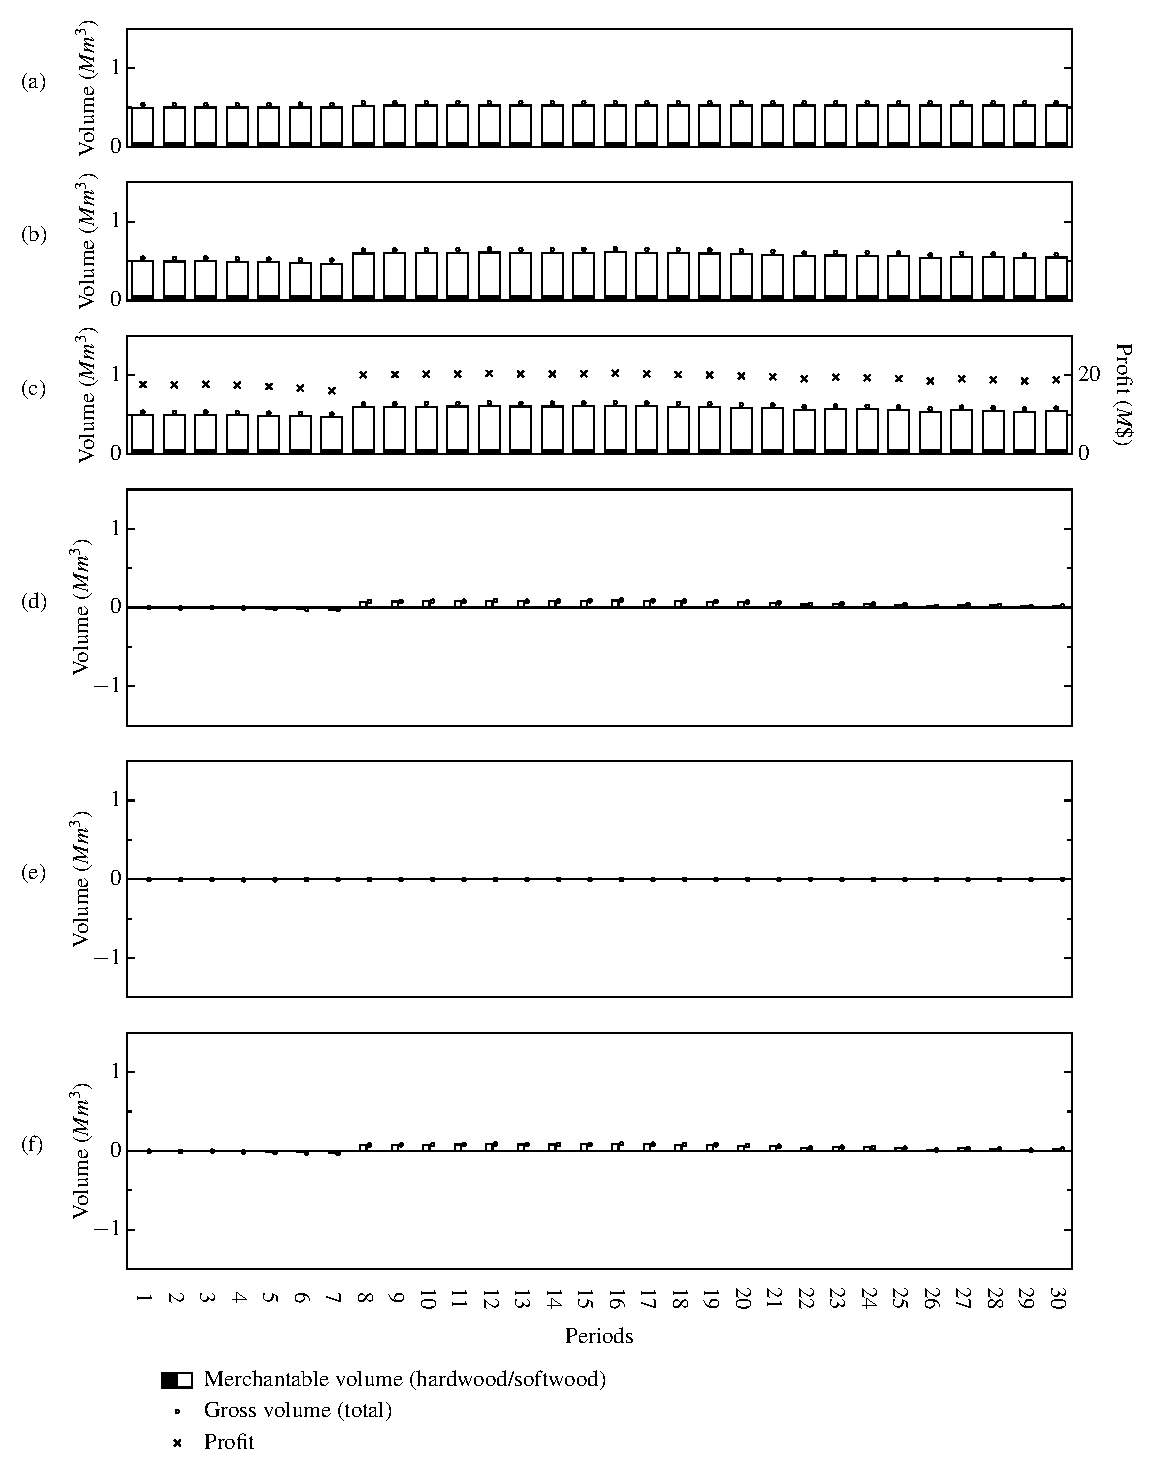
\includegraphics[width=0.65\columnwidth]{images/s3-2}
\end{figure}

\begin{table}[ht!]
\caption{Comparison of harvested volume and profit for periods 1--7 (scenarios 3.1 and 3.2)}
\label{tab:compare_volume-profit}
\renewcommand{\tabcolsep}{11pt}
\begin{tabular}{lrrrrrr}
\toprule
 & \multicolumn{2}{c}{Scenario 3.1} & \multicolumn{2}{c}{Scenario 3.2} & \multicolumn{2}{c}{Difference}\tabularnewline
Iteration & Volume & Profit & Volume & Profit & Volume & Profit\tabularnewline
 & (thousand $m^3$) & ($M\$$) & (thousand $m^3$) & ($M\$$) & ($\%$) & ($\%$)\tabularnewline
\midrule 
1 & 501 & 19.7 & 533 & 17.7 & 6 & -10\tabularnewline
2 & 507 & 19.9 & 530 & 17.6 & 5 & -11\tabularnewline
3 & 505 & 19.3 & 535 & 17.7 & 6 & -8\tabularnewline
4 & 496 & 18.5 & 525 & 17.5 & 6 & -5\tabularnewline
5 & 507 & 17.1 & 518 & 17.1 & 2 & 1\tabularnewline
6 & 527 & 15.1 & 516 & 16.7 & -2 & 11\tabularnewline
7 & 494 & 15.1 & 507 & 16.1 & 3 & 6\tabularnewline
\midrule 
Mean & 505  & 17.8 & 523 & 17.4 & 4 & -3 \tabularnewline
CV & 2 & 11 & 2 & 3 & 0 & -7 \tabularnewline
\bottomrule
\end{tabular}
\end{table}

% \section{Discussion}
% \label{sec:discussion}


As can be expected for scenario 1.1 (perfect implementation of
period-1 solution at each iteration), re-planned AAC solutions track
perfectly along initial optimal solution until a critical period is reached
(ie. period 7), after which AAC increases sharply and remains relatively
stable despite re-planning at each period, indicating negligible
influence of end-of-horizon effects on simulation results and low
systematic drift effect (SDE). The situation is noticeably different
for scenario 1.2 (imperfect implementation of first-period optimal
solution): AAC steadily declines until critical period, then increases sharply
after the critical period as new growing stock becomes available, and
resumes steady decline (see Figure \ref{fig:scenario1.2}(b)). This
\emph{declining non-declining yield} phenomenon is discussed in the
literature
\citep{mcquillan1986declining,daugherty1991credibility,gunn2007models},
however little has been done to address this issue in practice. Note
that documented cases of \emph{declining non-declining yield} in the
literature are all based on models with profit maximization objectives
(with even-flow constraints), whereas our model uses a volume
maximization objective (with even-flow constraints).

Scenarios 1.1 and 1.2 demonstrate that \emph{status quo} implementation of
the AAC model, if used within a \emph{status quo} rolling-horizon
hierarchical planning context, does not guarantee non-declining future
harvest levels \emph{even if the first period of optimal solution is
  implemented almost perfectly} and deterministic model assumptions
are assumed to hold. Undesirable behaviour of the AAC model under
these optimistic base-case conditions (ie. high level of coherence
between long- and short-term plans) shows that the \emph{status quo} planning
process is sensitive to even the smallest deviations from the
long-term optimal solution during its implementation. The infinite
demand assumption behind these first two scenarios is unrepresentative
of the \emph{status quo} planning context in many jurisdictions; harvest volumes
are generally well below AAC, and choice of harvest blocks may
include significant biases relative to optimal AAC solution
(ie. closest to access roads, least dispersed, etc).

Scenarios 2.1 and 2.2 simulate impact of incoherence between supply
and demand assumptions in planning models. For both scenarios,
species-wise demand distribution is a skewed subset of supply. We
project current demand forward in two different ways. Scenario 2.1
assumes constant demand pattern (ie. species-wise demand is not updated
at each rolling-horizon re-planning iteration). Scenario 2.2 assumes
proportional demand (ie. species-wise demand is updated at each
rolling-horizon re-planning iteration, always using 80\% and 40\% of
most recently calculated softwood and hardwood AAC). Scenario 2.1
simulates an unsustainable trajectory; Figure \ref{fig:scenario2.1}(c)
shows a wood supply failure in period 6, followed by regular wood
supply failures later in the planning horizon. These wood supply
failures are induced by systematic omission of hardwood-rich forest
units from short-term harvest plans, and are not predicted by the
long-term wood supply model. In fact, the long-term wood supply model
had been predicting \emph{increasing} AAC levels\footnote{Increasing
  AAC can be explained by unanticipated accumulation of growing stock
  in the forest, due to harvest levels systematically below AAC.} for
several rolling-horizon planning iterations when the first wood supply
failure occurs (see Figure \ref{fig:scenario2.1}(b)). Scenario 2.2
simulates less severe wood supply failures, in part because we allow
species-wise demand to scale up and down (as a proportion of current
AAC) at each rolling-horizon re-planning iteration, thereby ensuring
a certain adaptive coherence between supply and demand (despite
a systematic species-skewed gap between planned and implemented harvest levels).

Scenarios 3.1 and 3.2 demonstrate some potential advantages of
integrating long- and short-term planning. In our integrated model,
the long-term wood supply plan is driven by short-term value creation,
\emph{viz.} the  wood supply solution is iteratively adjusted until it
converges on an even-flow wood supply plan that maximizes first-period
profit. Note that process parameters have
been set in our model such that softwood processing is generally more
profitable than hardwood processing (consistent with current situation
in Quebec according to industry data). Scenario 3.1 shows a
significant decline in profits between periods 1 and 7 which we
explain by low hardwood demand relative to projected hardwood harvest
levels in the long-term wood supply plan: at every iteration, the short-term planning agent
systematically avoids harvesting (less profitable) hardwood-rich
stands. Lower-value hardwood growing stock accumulates, causing
a systematic decline of value-creation potential in the medium term;
this scenario is clearly not sustainable.

We added a simple constraint to the wood supply model in Scenario 3.2,
which sets an upper bound on long-term hardwood harvest projection
to (approximately) match hardwood demand in the value creation
network. The impact of improved coherence between long- and short-term
planning processes is obvious: optimizing long-term hardwood supply
planning to more closely match long-term demand eliminates much of the
softwood high-grading behaviour observed in scenario 3.1,
resulting in stabilized profit and volume flow, and increased mean AAC
for the first seven planning iterations (see Figures
\ref{fig:scenario3.1}(c) and \ref{fig:scenario3.2}(c), and Table
\ref{tab:compare_volume-profit}).

The last five scenarios all exhibit some form of \emph{systematic
  drift effect} (SDE) that is not predicted by the long-term wood
supply optimization model. Evidence of SDE in our illustrative case
study includes a monotonic increase or decrease in AAC over several
iterations, a monotonic change in AAC composition (ie.  ratio of
hardwood to softwood), increasing incoherence between supply and
demand, and increasing infeasibility of the demand-satisfaction problem
(ie. instability of simulated harvest levels). Undetected forms of
drift are likely to exist within these scenarios for performance
indicators not presented here (eg. standing timber inventory, age
class distribution, landscape patch distribution, value-creation
potential, harvest block size and location distribution, wildlife
habitat suitability, etc).


\section{Conclusion}
\label{sec:conclusion1}

The illustrative case study presented here shows that the \emph{status quo}
hierarchical forest planning process (ie. two-phase rolling-horizon
iterative re-planning) is incoherent and dysfunctional: it fails to
demonstrate long-term sustainability of government-endorsed short-term
harvest levels, fails to reliably meet industrial fiber demand over
time, and exacerbates incoherence between wood supply and fiber demand
over several planning iterations. We identify systematic differences
between planned and actual harvesting activities as an important
factor contributing to this dysfunction, which manifests itself as
either instability in long-term wood supply or lost short-term value
creation opportunity.

We show that coherence between long- and short-term planning solutions
can be improved significantly by manipulating linkages between
planning levels (eg. adding species-wise demand constraint to the AAC
model). Although simplistic in its implementation, our integrated
model illustrates the potential value (in terms of both credibility of
long term planning process and performance of short-term planning
process) of anticipating short-term planning objectives (eg. demand
satisfaction) within a long-term planning model. Based on our
preliminary simulation results, we feel there is much potential for
further refinement of linkages between long- and short-term planning processes.

Much of the difference between planned and actual harvesting activities
can be explained by the principal-agent relationship between
government and industry planners. This principal-agent relationship
could potentially be modelled as a bi-level optimization problem, and
the long-term planning process extended to include an
anticipative-iterative dimension. This would allow the principal to
develop long-term forest policy that is more likely to be compatible
with anticipated agent behaviour, thereby inducing a reduction in SDE, and
improving hierarchical planning process credibility and value-creation potential.

% We propose changes to the long-term planning process that
% may produce more effective contracts, thus reducing the gap between
% projected and actual agent behaviour, thereby improving credibility of
% government policy as a tool for ensuring long-term sustainability of
% forest resources. Furthermore, more efficiently designed contract
% between principal and agent may reduce pressure on constraints and
% incentives required to achieve desired outcome from the planning
% process, thereby providing a more flexible and agile short-term
% planning environment for the agent. In other words, an optimal design
% for the hierarchical forest management process ensures long-term
% sustainability of the forest resource while providing maximum
% short-term value-creation opportunity for the forest industry.

\section{Acknowledgements}

This study was supported by funding from the \emph{FORAC Research
  Consortium} and the \emph{Fonds de recherche du Qu\'{e}bec -- Nature
  et technologies}. The authors would like to thank
Dr. Fr\'{e}d\'{e}ric Raulier and the two anonymous reviewers for their
valuable comments and suggestions during the writing process, which
greatly helped improve the quality of this paper.

\bibliographystyle{plainnat}
\bibliography{phd}


%%% Local Variables: 
%%% mode: latex
%%% TeX-master: "909303058"
%%% End: 